\documentclass[a0,portrait]{a0poster}

\usepackage{multicol}
\usepackage{multirow}

\columnsep=100pt

\columnseprule=3pt

\usepackage[svgnames]{xcolor} 

\usepackage{palatino}

\usepackage{lineno}
\usepackage{verbatim}
\usepackage{mathptmx}
\usepackage{color}
\renewcommand{\familydefault}{\rmdefault}

\usepackage{url}
\usepackage{cite}
\renewcommand{\thefootnote}{\roman{footnote}}

\usepackage{graphicx} % Required for including images
\graphicspath{} % Location of the graphics files
\usepackage[font=small,labelfont=bf]{caption} % Required for specifying captions to tables and figures
\usepackage{amsfonts, amsmath, amsthm, amssymb} % For math fonts,
                                % symbols and environments

\makeatother

\DeclareMathOperator{\samesign}{same-sign}
\DeclareMathOperator{\oppositesign}{opposite-sign}

\definecolor{VUdarkred}{rgb}{0.48235, 0, 0.24706}

\newcommand{\uline}[1]{\underline{#1}}
\newcommand{\address}[1]{\centerline{#1}}
%\newcommand{\rightaddress}[1]{\centerline{\small #1}}

\newcommand{\GeVns}{~\mathrm{GeV}} 
\newcommand{\ET}{E_\mathrm{T}}
\newcommand{\unit}[1]{~#1}
\newcommand{\abs}[1]{|#1|}
\newcommand{\pt}{p_\mathrm{T}}
\newcommand{\GeV}{~\mathrm{GeV}}
\newcommand{\mum}{~$\mu$m\ }
\newcommand{\mus}{~$\mu$s\ }
\newcommand{\tab}{$\phantom{x}$\quad}
\newcommand{\tabc}{$\phantom{x}$\quad$\circ$\ }

\begin{document}

%=============================
%Header
%=============================
\begin{minipage}[b]{0.1\linewidth}
\begin{flushleft}

\includegraphics[width=\linewidth]{VU_Logo_bordo.png}\\[0.5cm]$\phantom{x}$
\end{flushleft}
\end{minipage}
%
\hspace{1cm}
%
\begin{minipage}[b]{0.67\linewidth}
{\begin{centering} \Huge \color{VUdarkred} 
\title \textbf{Drell-Yan Process Analysis Using 2016 CERN CMS Proton-Proton Collision Data}
\bigskip
\color{Black}
\end{centering}
}\\ % Title
{\Large \textbf{\uline{Marijus\ Ambrozas},
 Andrius Juodagalvis}
}\\[0.5cm] % Author(s)
Institute of Theoretical Physics and Astronomy, Vilnius University, Vilnius, Lithuania\\[0.4cm] % University/organization
{\small \textit{e-mail:} \texttt{marijus.ambrozas@ff.stud.vu.lt} }\\
\end{minipage}
%
\hspace{1cm}
%
\begin{minipage}[b]{0.19\linewidth}
\begin{flushright}

\includegraphics[width=\linewidth]{VUFF-TFAI-logo.jpg}\\[0.8cm]$\phantom{x}$
\end{flushright}
\end{minipage}
%\hspace{8mm}

\vspace{-0.8cm} 

\begin{multicols}{2}

\small

%\linenumbers

\section*{Introduction}
%Proton structure, PDFSs
\begin{centering}
	\begin{minipage}{0.63\linewidth}
		High energy proton-proton collisions reveal that protons are not point-like but rather have an inner structure, consisting
		of ``partons'' -- quarks and gluons.
		Theoreticians describe this structure using parton distribution functions (PDFs) $f_i(x, Q^2)$, that tell the
		probability density of detecting a parton $i$, which is carrying a fraction $x$ of proton's longitudinal momentum
		at the energy scale $Q$.
		The cross section of a specific event, that could occur during the pp collision can be calculated by combining
		the PDFs of both protons together with parton-parton interaction cross section:
		\begin{equation}
			\label{eq:SigmaFromPDFs}
			\sigma = \sum_{i, j} \int \mathrm{d}x_1 \int \mathrm{d}x_2 \,
			f_{i}(x_1, \, Q^2) \, f_{j}(x_2 \, Q^2) \, \hat{\sigma}(x_1 p_1, \, x_2 p_2, \, Q^2) \; \mathrm{.}
		\end{equation}
		The possibility of interactions between ``sea quarks'' gets bigger with higher and higher $Q$.
		High-energy pp collisions, such as those produced at the LHC in CERN allow us to witness these rare events.
		Though, very precise knowledge of PDFs is required in order to describe these observations theoretically.
		Since PDFs are not predicted by quantum chromodynamics (QCD), they are obtained from various experimental
		measurements \cite{PDFs}.
		
		\vspace{1cm}
				
		\textbf{Drell-Yan} (DY) process is a quark-antiquark annihilation resulting in a lepton-antilepton pair.
		This process is described in the standard model by s-channel exchange of a virtual photon or $Z$ boson:
		\begin{equation*}
			q\bar{q}\rightarrow Z/\gamma^{*}\rightarrow l^{+}l^{-} \; .
		\end{equation*}
		Theoretical predictions of the DY differential cross section are established up to next-to-next-to-leading
		order (NNLO) in perturbative QCD.
		Comparison between the theoretical predictions and precise experimental measurements allows scientists to
		constrain the PDFs, test perturbative QCD and validate the predictions of higher order corrections.
		Also, DY study is important for other physics analysis at the LHC, where the DY lepton-pair production is
		a major source of background \cite{DYRidhi}.
		
		\vspace{0.5cm}
		The event selection is performed first in the measurement to constrain the phase space in such a way that the
		contribution of various background sources is reduced.
		However, contribution of backgrounds cannot be fully suppressed and still must be considered in DY differential
		cross section measurements.
		The most significant genuine lepton backgrounds are $t\bar{t}$, $WW$, $WZ$, $tW$, $\bar{t}W$, $ZZ$.
		$\mathrm{DY}\rightarrow\tau\tau$ is also considered a background in studies of DY electron-pair and muon-pair production 
		(called electron channel and muon channel respectively).
		There is also a contribution of fake lepton backgrounds from processes, such as $W+\mathrm{Jets}$ and $QCD$ (multijet).
		Since only the long-living final-state particles can be detected, there is no simple way to differentiate between
		a Drell-Yan and a background event.
		It is only possible to get a statistical estimate of the number of background events.
		The estimation for background could be obtained from Monte Carlo (MC) simulation or using data-driven techniques,
		which rely on both measurement and MC.
		Data-driven methods are often preferred over MC in order to reduce simulation-related uncertainties, such as
		cross-section uncertainties of various processes or imperfect simulations of detector's response.
		ABCD and fake rate methods are commonly used to estimate the contribution of fake lepton backgrounds, while $e\mu$
		method is used for real lepton background estimation.
		The event selection procedures and background estimation using $e\mu$ method will be discussed further in the presentation.
	\end{minipage}
	\hfill
	\begin{minipage}{0.33\linewidth}\centering
		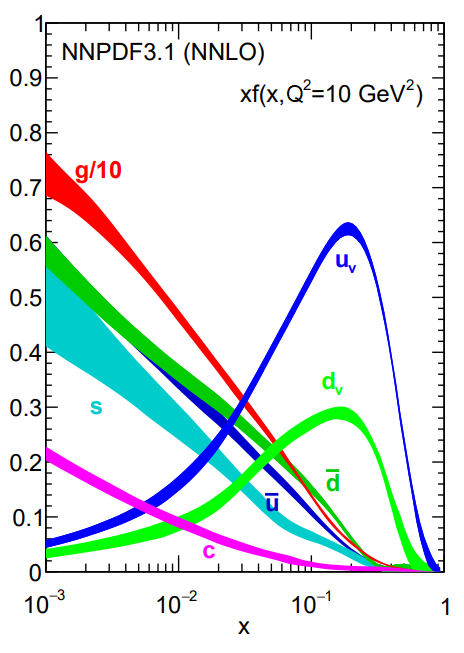
\includegraphics[width=0.8\linewidth]{NNPDF10.PNG}
		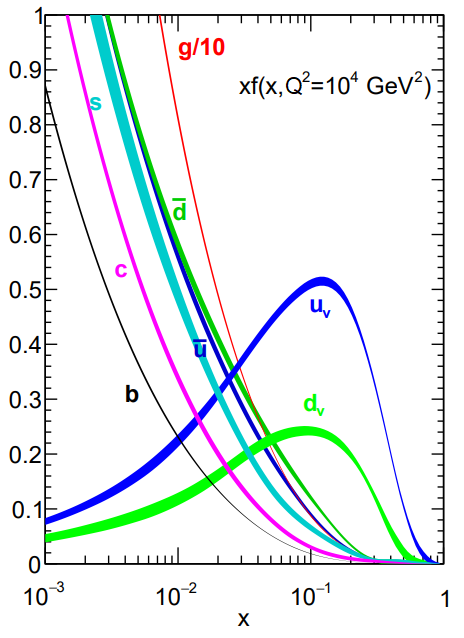
\includegraphics[width=0.8\linewidth]{NNPDF10000.PNG}
		\vspace{-0.9cm}
		\captionof{figure}{\label{fig:PDFs}
			Two examples of NNPDF3.1 parton distribution functions at $Q^{2}\!=\!10$ $\mathrm{GeV}^{2}$ (top) and
			$Q^{2}\!=\!10^{4}$ $\mathrm{GeV}^{2}$ (bottom) \cite{NNPDF}.
			Note the rise in probability densities of partons with small $x$ when moving to higher energy scale.
		}
		
		\vspace{0.5cm}
		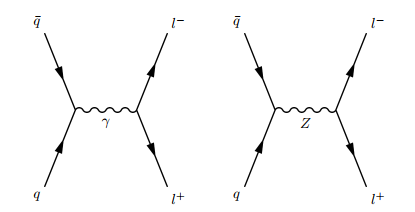
\includegraphics[width=\linewidth]{DYprocess.PNG}
		\vspace{-0.5cm}
		\captionof{figure}{\label{fig:DYproc}
			Feynman diagrams showing the Drell-Yan process.
		}
	\end{minipage}
\end{centering}

\vspace{-0.2cm}
\section*{The CMS detector}
\vspace{-0.2cm}
The Compact Muon Solenoid (CMS) is a multi-purpose particle detector.
It is able to detect many different types of particles produced by collisions happening in the LHC.
The CMS detector is 21 metres long, 15 metres wide and tall, and weights $14,000$ tonnes.
The main component of CMS is the superconducting solenoid electromagnet which can produce a magnetic field of $4$ T.
CMS consists of multiple types of subdetectors, each of them having barrel and endcap constituents.

\vspace{0.5cm}
\begin{centering}
	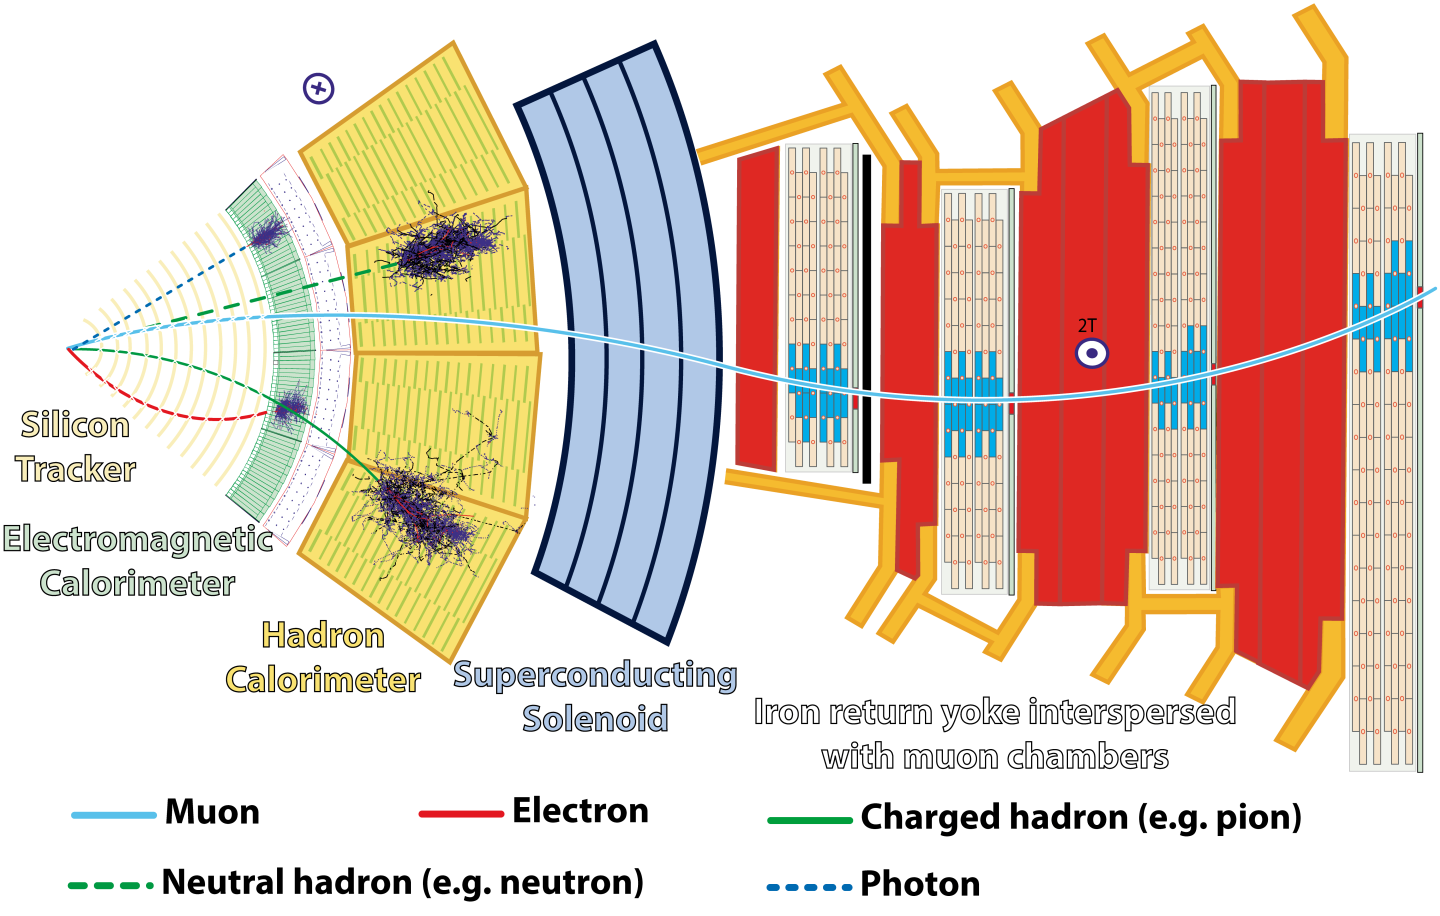
\includegraphics[width=0.8\linewidth]{CMSslice.png}
	\vspace{-0.5cm}
	\captionof{figure}{\label{fig-CMSslice}
		The transverse view through CMS showing different parts of the detector \cite{CMSslice}.
		The different colour lines represent the trajectory of particles emerging from the collision.
		The dashed line means that the particle has no electric charge and thus does not leave its track inside the tracker.
	}
\end{centering}
\vspace{0.5cm}

\noindent All the subdetectors have their own purpose are laid out in a specific order to maximize their efficiency.
Moving from the inside out you can find the silicon tracker, which captures tracks of charged particles, electromagnetic
calorimeter (ECAL), that detects electrons and photons, hadron calorimeter (HCAL), which detects hadrons, the
superconducting solenoid, that creates a strong magnetic field that curves the tracks of charged particles,
and muon chambers, which capture muon tracks, interleaved with the return yoke, that confines the high magnetic
field to the volume of the detector \cite{CMSdetector}.

\noindent In 2016 CMS detector has captured $35.9$ $\mathrm{fb}^{-1}$ of pp collision data.
That is around $2 \cdot 10^{15}$ events (and about $10$ times more than captured in 2015)!
This allows us to have very small statistical uncertainties, but at the same time makes it difficult to store such vast amounts
of data and to perform the analysis procedures quickly.

\vspace{-0.6cm}
\section*{Event selection}
\begin{minipage}{0.46\linewidth}
	This Drell-Yan analysis focuses only on 1D differential cross section $\mathrm{d}\sigma/\mathrm{d}m_{ll}$ measurement.
	It was performed using 2016 CMS data and includes only the DY electron-pair and muon-pair production.
	MC datasets, corresponding to signal ($\mathrm{DY}\rightarrow ll$), and various background processes ($t\bar{t}$, $WW$, $WZ$,
	$tW$, $\bar{t}W$, $ZZ$, $W+\mathrm{Jets}$ and $QCD$) were also used for comparison with the observed data and background estimation.
	The pre-produced datasets that were used for the analysis take up around $14$ TB of storage.
	The event selection criteria were specifically chosen so that events that pass the selection are mostly DY events.
	The criteria were different for the electron and muon channels.
	They are provided in more detail in table \ref{table:Selection}.
	In order to reduce the time of further analysis, new data files, containing only the most necessary information and only the
	selection-passing events, were created.
	Newly created files are just around $14$ GB in size.
	The whole event selection procedure took nearly 4 days.
\end{minipage}
\hfill
\begin{minipage}{0.52\linewidth}
	\vspace{-0.8cm}
	\centering
	\captionof{table}{\label{table:Selection}
		Selection criteria for electron and muon channels.
	}
	\vspace{-0.8cm}
	\begin{tabular}{|c|c|}
		\hline 
		\multirow{2}{12em}{\centering \textbf{Electron channel}} &
			\multirow{2}{12em}{\centering \textbf{Muon channel}} \\
		& \\
		\hline \hline
		\rule{0pt}{22pt}		
		\multirow{3}{12em}{\centering \textbf{Trigger}: HLT\_Ele23\_Ele12} &
			\multirow{3}{12em}{\centering \textbf{Trigger}: HLT\_IsoMu24 OR HLT\_IsoTkMu24 (using trigger matching)} \\
		& \\
		& \\
		\hline
		\rule{0pt}{24pt}
		\multirow{4}{12em}{\centering $p_{\mathrm{T}}^{\mathrm{Lead}}>28$ GeV,\\ $p_{\mathrm{T}}^{\mathrm{Sublead}}>17$ GeV,\\
						   $|\eta_{\mathrm{SC}}|<2.4$, \textbf{excluding} $1.4442<|\eta_{\mathrm{SC}}|<1.566$} &
			\multirow{4}{12em}{\centering $p_{\mathrm{T}}^{\mathrm{Lead}}>28$ GeV,\\ $p_{\mathrm{T}}^{\mathrm{Sublead}}>17$ GeV,\\
						   	   $|\eta_{\mathrm{SC}}|<2.4$} \\
		& \\
		& \\
		& \\
		\hline
		\rule{0pt}{22pt}		
		Electron MediumID &	Muon TightID, $I_{\mathrm{PF}}^{\mathrm{Rel.}}<0.15$ \\
		\hline
		\rule{0pt}{22pt}
		\multirow{4}{12em}{\centering Exactly two electrons passing the event selection (no opposite sign requirements)} &
			\multirow{4}{12em}{\centering Two \textbf{opposite sign} muons with smallest vertex fit $\chi^2<20$,\\ 3D angle $<\pi-0.005$ rad} \\
 		& \\
 		& \\
 		& \\
		\hline
	\end{tabular}
\end{minipage}
\vspace{0.2cm}

\noindent MC events have to be normalized to observed integrated luminosity and undergo several corrections because of
the differences between simulated and real experiment conditions, before we can compare them with experimental data or
use in data-driven background estimation techniques.
The corrections include: pileup correction, electron energy scale correction, muon momentum scale correction, various
efficiency scale factors, primary vertex $z$ position correction and level 1 trigger pre-firing correction.

\section*{Background estimation}
So far in this analysis only real dilepton background ($\mathrm{DY}\rightarrow\tau\tau$, $t\bar{t}$, $WW$, $tW$,
$\bar{t}W$) yield was estimated from data.
This was done using $e\mu$ method, which works as follows:
If we create two heavy particles, which can decay into leptons flavour-symmetrically, and we do
not consider the decay into a $\tau$ lepton, we can have four different final states, for example: $WW\rightarrow e^{+}e^{-}$,
$WW\rightarrow \mu^{+}\mu^{-}$, $WW\rightarrow e^{+}\mu^{-}$, $WW\rightarrow \mu^{+}e^{-}$.
In an ideal scenario, the ratio between a number of $ee$ (or $\mu\mu$) final state events and a number of $e\mu$ final state
events should be $1/2$.
Though, for us it is enough to make an assumption that this ratio stays the same for measurement and MC, regardless of
what its value actually is: $N_{ee}^{\mathrm{Data}}/N_{e\mu}^{\mathrm{Data}}=N_{ee}^{\mathrm{MC}}/N_{e\mu}^{\mathrm{MC}}$.
This can be seen as an equation.
The $e\mu$ event sample contains only background events, since $e\mu$ final state is not possible for the Drell-Yan process.
This means that if we solve the given equation for $N_{ee}^{\mathrm{Data}}$, we get a data-driven estimate for the number
of $ee$ final state background events:
\begin{equation}
	\label{eq:EMuMethod}
	N_{ee}^{\mathrm{Est.}}=\frac{N_{ee}^{\mathrm{MC}}}{N_{e\mu}^{\mathrm{MC}}}\cdot N_{e\mu}^{\mathrm{Data}} \; .
\end{equation}
The same statement would hold if we swap $ee$ with $\mu\mu$.

\noindent However, it is known, that the $e\mu$ sample is contaminated with a small part of fake $e\mu$ events: mostly $W+\mathrm{Jets}$
and $QCD$ (from $b\bar{b}$ decays).
Since these are fake lepton events (a fast jet is misreconstructed as a lepton), they are not suitable for use in $e\mu$ method
and their effect on $ee$ ($\mu\mu$) background estimation has to be reduced.
In this work, the $e\mu$ $W+\mathrm{Jets}$ background was estimated from MC, while $e\mu$ $QCD$ background was estimated using
a data-driven method.
Events, where reconstructed electron and muon have the same electrical charge, were selected for $QCD$ estimation.
Then, the remainder left after subtracting simulated real lepton and $W+\mathrm{Jets}$ yields from the observed same-sign
distribution was expected to consist of just $QCD$ events.
The obtained same-sign $QCD$ distribution was transformed into the opposite-sign distribution by dividing the number of
same-sign events by a constant $R\approx 0.57$, which can be calculated theoretically.
This way, we get:
\begin{equation}
	\label{eq:QCDest}
	N_{QCD \; \mathrm{\oppositesign}}^{\mathrm{est.}} = \frac{1}{R} \left( N^{\mathrm{Data}} - N_{\mathrm{DY}\rightarrow\tau\tau}^{\mathrm{MC}} -
	N_{t\bar{t}}^{\mathrm{MC}} - N_{WW}^{\mathrm{MC}} - N_{WZ}^{\mathrm{MC}} - N_{tW}^{\mathrm{MC}} - N_{\bar{t}W}^{\mathrm{MC}} -
	N_{ZZ}^{\mathrm{MC}} - N_{W+\mathrm{Jets}}^{\mathrm{MC}} \right)_{\mathrm{\samesign}} \; .
\end{equation}
Having done that, the obtained value for $QCD$ events could be subtracted from observed opposite-sign data.
Then the number of $e\mu$ data events should also be reduced by an amount $1/1+C$, where
\begin{equation*}
	C = \frac{ N_{W+\mathrm{Jets}}^{\mathrm{MC}} } { N_{\mathrm{DY}\rightarrow\tau\tau}^{\mathrm{MC}} + 
	N_{t\bar{t}}^{\mathrm{MC}} + N_{WW}^{\mathrm{MC}} + N_{WZ}^{\mathrm{MC}} + N_{tW}^{\mathrm{MC}} + N_{\bar{t}W}^{\mathrm{MC}} +
	N_{ZZ}^{\mathrm{MC}} + N_{W+\mathrm{Jets}}^{\mathrm{MC}} } \; ,
\end{equation*}
to account for $W+\mathrm{Jets}$ contamination.

\section*{Results}

Electron-muon final state events were selected with combined selection criteria from both $ee$ and $\mu\mu$ channels:
electron had to satisfy the criteria presented in the left column of table \ref{table:Selection}, while muon had to satisfy
the criteria presented in the right column.
Though, only single muon trigger was used in $e\mu$ selection (no electron trigger).
Same-sign electron-muon invariant mass distribution is presented in figure \ref{fig:emu_SS}.
A significant contribution from $W+\mathrm{Jets}$ background is predicted by MC, but there is still a big discrepancy between
data and MC in the given distribution.
This was necessary to estimate the $e\mu$ $QCD$ background, which is included into the opposite-sign $e\mu$ invariant mass
histogram in figure \ref{fig:emu_wQCD}.
The amount of $QCD$ background is clearly not trivial and taking that into consideration should allow us to estimate the
number of DY background events more correctly.

\begin{centering}
	\vspace{0.6cm}
	\begin{minipage}[t]{0.48\linewidth}
		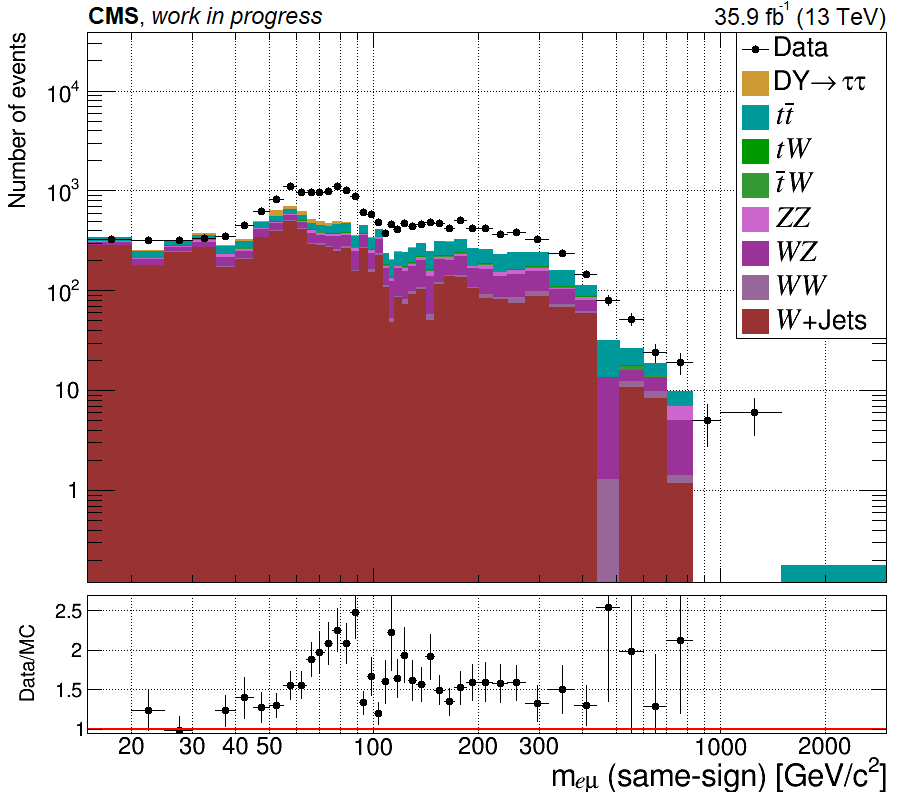
\includegraphics[width=0.99\linewidth]{EMuSS_mass_1.png}
		\vspace{-0.7cm}
		\captionof{figure}{\label{fig:emu_SS}
			$e^{\pm}\mu^{\pm}$ invariant mass spectrum.
			Black dots represent 2016 CMS data while the colored bars represent MC simulated events from different processes.
			The scales are logarithmic.
		}
	\end{minipage}
	\hfill
	\begin{minipage}[t]{0.48\linewidth}
		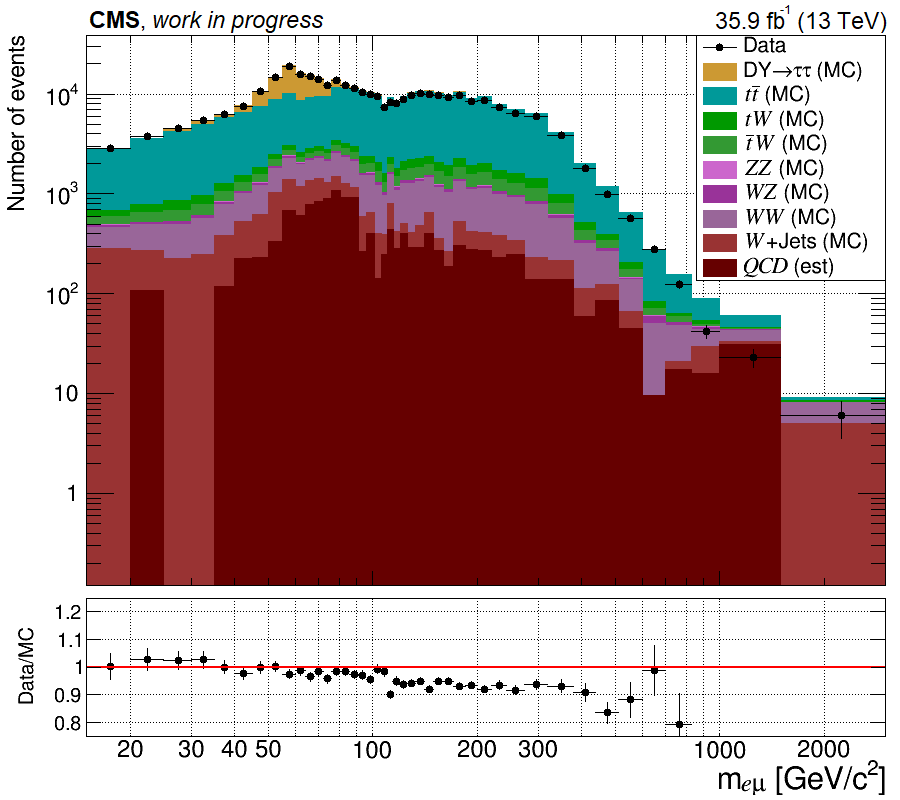
\includegraphics[width=0.99\linewidth]{EMu_mass_wQCD_1.png}
		\vspace{-0.7cm}
		\captionof{figure}{\label{fig:emu_wQCD}
			$e^{\pm}\mu^{\mp}$ invariant mass spectrum.
			Markings and scale are the same as in fig.\ \ref{fig:emu_SS}.
			The $QCD$ yield was estimated from the discrepancy between data and MC in figure \ref{fig:emu_SS} using \eqref{eq:QCDest}
			formula.
		}
	\end{minipage}
\vspace{0.8cm}
\end{centering}

\noindent However, the $\mathrm{Data/MC}$ distribution presented in the bottom of figure \ref{fig:emu_wQCD} still shows some unexpected
behaviour: in ideal scenario, values of the given ratio should be randomly distributed around $1$, but here the values seem to have
a systematic shift depending on the mass value.
This will also increase the systematic uncertainty of DY dielectron background estimation, which is shown in figure \ref{fig:EEest}.
Here we can see that ratio between the data-driven estimation and MC shows the same behaviour as the $e\mu$ $\mathrm{Data/MC}$
distribution.
This results in a higher difference between CMS data and combined estimations (either data-driven or MC) in high-mass regions
of the full dielectron invariant mass spectrum, shown in figure \ref{fig:EEfinal}.
Very similar results are obtained in dimuon channel as well.
Since the most dominant process in the $e\mu$ channel is $t\bar{t}$, one of the possible ways to reduce this systematic shift
could be top quark $p_{\mathrm{T}}$ reweighting.
Another way to improve the result could be the estimation of both $W+\mathrm{Jets}$ and $QCD$ backgrounds from data, since simulated
$W+\mathrm{Jets}$ distributions are very sensitive to statistical fluctuations due to very small acceptance and very big cross section.
Systematic uncertainty evaluations should be made after including both of the suggested improvements in the nearest future.

\begin{centering}
	\vspace{0.6cm}
	\begin{minipage}[t]{0.48\linewidth}
		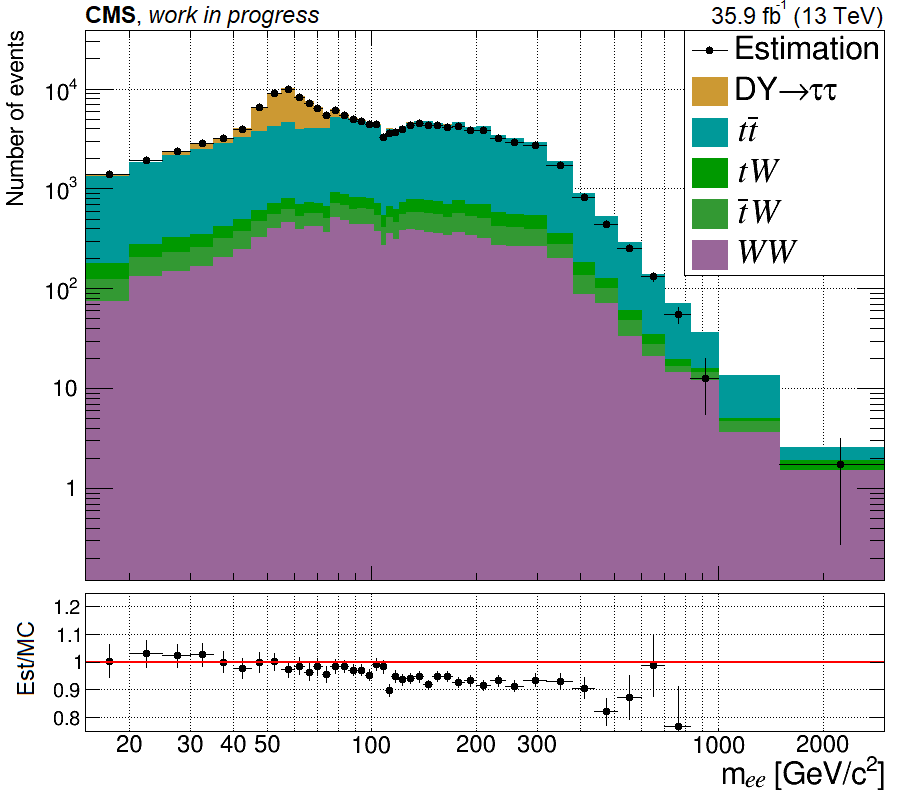
\includegraphics[width=0.99\linewidth]{EE_mass_est_1.png}
			\vspace{-0.7cm}
			\captionof{figure}{\label{fig:EEest}
			Dielectron invariant mass distribution of $\mathrm{DY}\rightarrow ee$ backgrounds estimated using $e\mu$ method.
			Black dots represent data-driven estimation while the colored bars represent MC events corresponding to different processes.
		}
	\end{minipage}
	\hfill
	\begin{minipage}[t]{0.48\linewidth}
		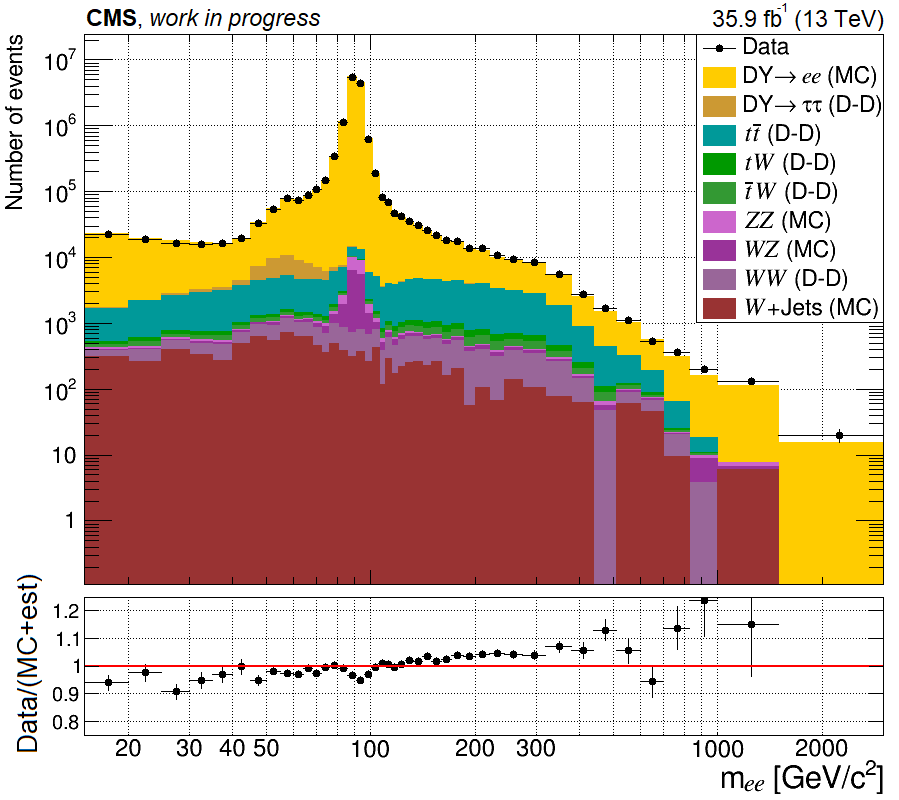
\includegraphics[width=0.99\linewidth]{EE_mass_final_1.png}
		\vspace{-0.7cm}
		\captionof{figure}{\label{fig:EEfinal}
			The resultant dielectron invariant mass spectrum.
			Black dots represent real data while the colored bars represent either data-driven estimations (where possible) or
			MC simulated events from different processes.
			The $QCD$ process is not yet included.
		}
	\end{minipage}
\end{centering}
\vspace{0.5cm}

\noindent The presented work could have not been done without student's scientific practise project (no. 09.3.3-LMT-K-712-10-0128),
funded from EU Structural Funds.
The work was made in collaboration with researchers from Seoul National University and University of Nebraska-Lincoln.

\begin{thebibliography}{References}
	\vspace{-0.5cm}
	\bibitem{PDFs} Ringail\.{e} Pla\v{c}akyt\.{e}, Parton Distribution Functions, Proceedings, PIC 2011 (2011).
	
	\bibitem{DYRidhi} Ridhi Chawla, Differential cross-section measurement of the Drell-Yan process at 13 TeV proton-proton
	collisions with the CMS detector, Springer Proc.\ Phys.\  \textbf{203}, 349 (2018).	
	
	\bibitem{NNPDF} The NNPDF Collaboration, Parton distributions from high-precision collider data, CAVENDISH-HEP-17-06 (2017).

%	\bibitem{DY_CMSPAS}CMS Collaboration, Measurement of differential Drell-Yan cross section in proton-proton collisions at 13 TeV,
%	CMS-PAS-SMP-16-009 (2016).

	\bibitem{CMSdetector} The CMS Collaboration, The CMS experiment at the CERN LHC, JINST 3 S08004 (2008)

	\bibitem{CMSslice} David Barney, CMS Detector Slice, CMS-PHO-GEN-2016-001 (2016)

\end{thebibliography}

\end{multicols}

\end{document}